\section{Simulating the data and the model} \label{sec:simulation}
\subsection{The data}
\comm{Challenges:
- estimating parameters based on simulated data might not give the correct estimations}

The field experiment originally collected data on 1,440 daily impressions, clicks and orders for 36 keywords over a 40-day period from June 2009 to July 2009.\footnote{Though distinguishing between the biases of the factors and the data itself may seem straight forward (like $\theta^k_1$ times $Adpos_{kt}$), the authors didn't clearly allude in their estimations to either the Greek letters (the biases) or the roman words (the data). Interpreting the exact model with its parameters has thus been a challenge. The group has arrived at the conclusion to treat table 2 on page 40 as the data and tables 4, 5, 7 and 8 on  pages 41f. as mean values for the parameter estimates.}
To follow the model, data has been simulated based on the keyword performance summary statistics \citep[table 2 on p. 40]{agarwal_organic_2015}. Figure \ref{fig:Data} gives an overview to the distributions assumed.\\
The code below shows the simulation in R. With the help of the package \texttt{rtruncnorm}, the max and min values from figure \ref{fig:Data} could be taken into account as well.\footnote{The full code can be found in the appendix.}

\begin{lstlisting}[caption={Simulating the data}]
library(rtruncnorm)
## instantiate the values to estimate
num_keywords <- 36
num_days <- 40
num_observations <- 1440

# Poisson impressions
impressions <- matrix(round(rpois(n=num_observations, lambda = rep(72.8, num_observations)), 0), nrow=num_keywords, ncol=num_days)
impressions[impressions > 1666] <- 1666
impressions[impressions < 1] <- 1

# [removed clicks and orders for this example as they were poisson-distributed as well]

# Normally distributed data with organic being binomial distributed
organic <- matrix(rbinom(n=num_observations, size = 1, p=0.15),
                  nrow=num_keywords, ncol=num_days)
iv_organic <- matrix(round(rtruncnorm(n=num_observations, a=0.1, b=2.34, mean=0.42, sd=0.23),2), nrow=num_keywords, ncol=num_days)
# [removed sponsored_comp, iv_sponsored and lq_score and bid as they are normally distributed and constructed the same way]

# Binomial distributions of brand and specificity
brand <- matrix(rbinom(n=num_keywords, size = 1, p=0.6),
                nrow=num_keywords, ncol=1)

specificity <- matrix(rbinom(n=num_keywords, size=1, p=0.4),
                      nrow=num_keywords, ncol=1)

\end{lstlisting}

\begin{figure}
    \centering
    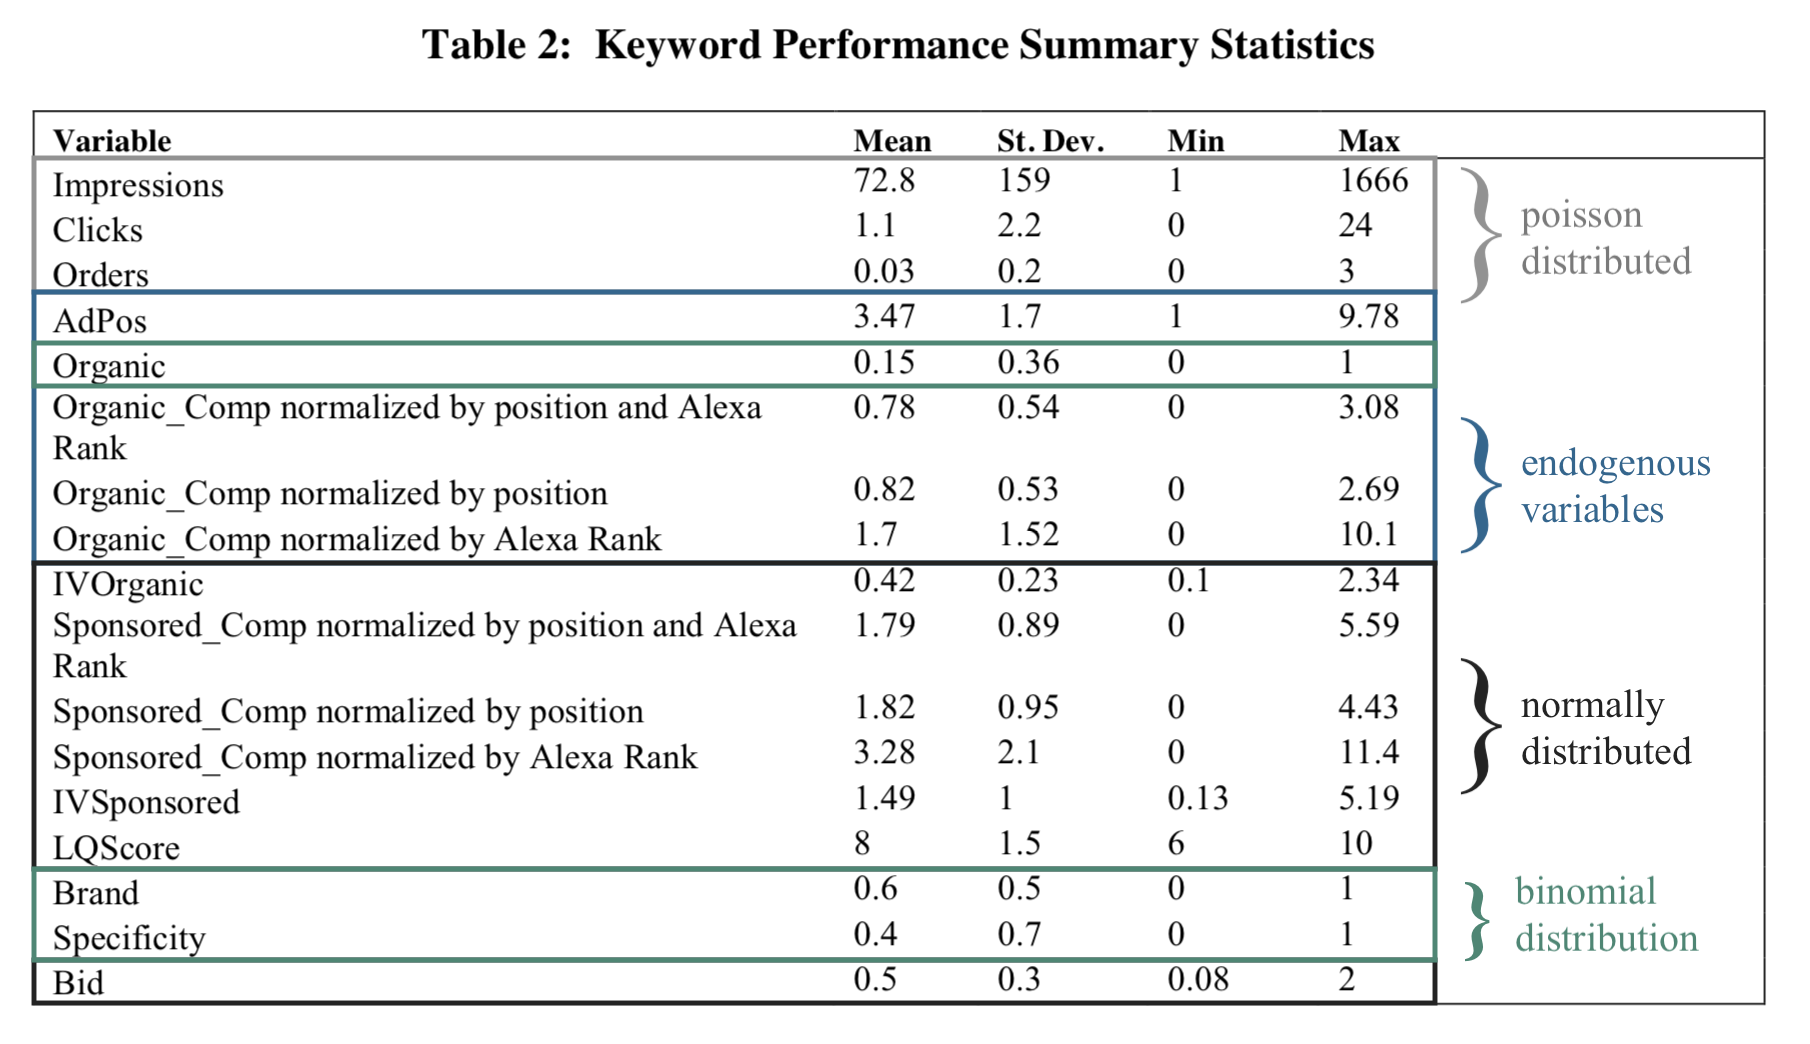
\includegraphics[scale=0.35]{Data}
    \caption{The summary statistics for the original data, including its interpreted distributions.\protect\footnotemark}
    \label{fig:Data}
\end{figure}
\footnotetext{The endogenous variables $AdPos_{kt}$ and $OrganicComp_{kt}$ were listed in this list, though contradicting the notion of "data".}

\subsection{The Distributions}
As shown in figure \ref{fig:Data}, the simulated variables follow a variety of distributions. Since the authors do not explicitly state which type of distribution each data item follows, we have assumed the most likely distribution based on the values provided in the summary statistics table. To this end, we simulated a total of 13 variables (we only focused on Sponsored Competition normalized by both position and Alexa Rank), the variable counts for each type of distribution being as follows: 
\begin{itemize}
    \item 3 Poission-distributed
    \item 3 Binomial-distributed
    \item 7 Normally distributed
\end{itemize}
The density distributions for each of these variable sets are described in figure \ref{fig:Poission}.
\subsubsection{Poisson-Distributed Variables}
\begin{figure}[!h]
    \centering
    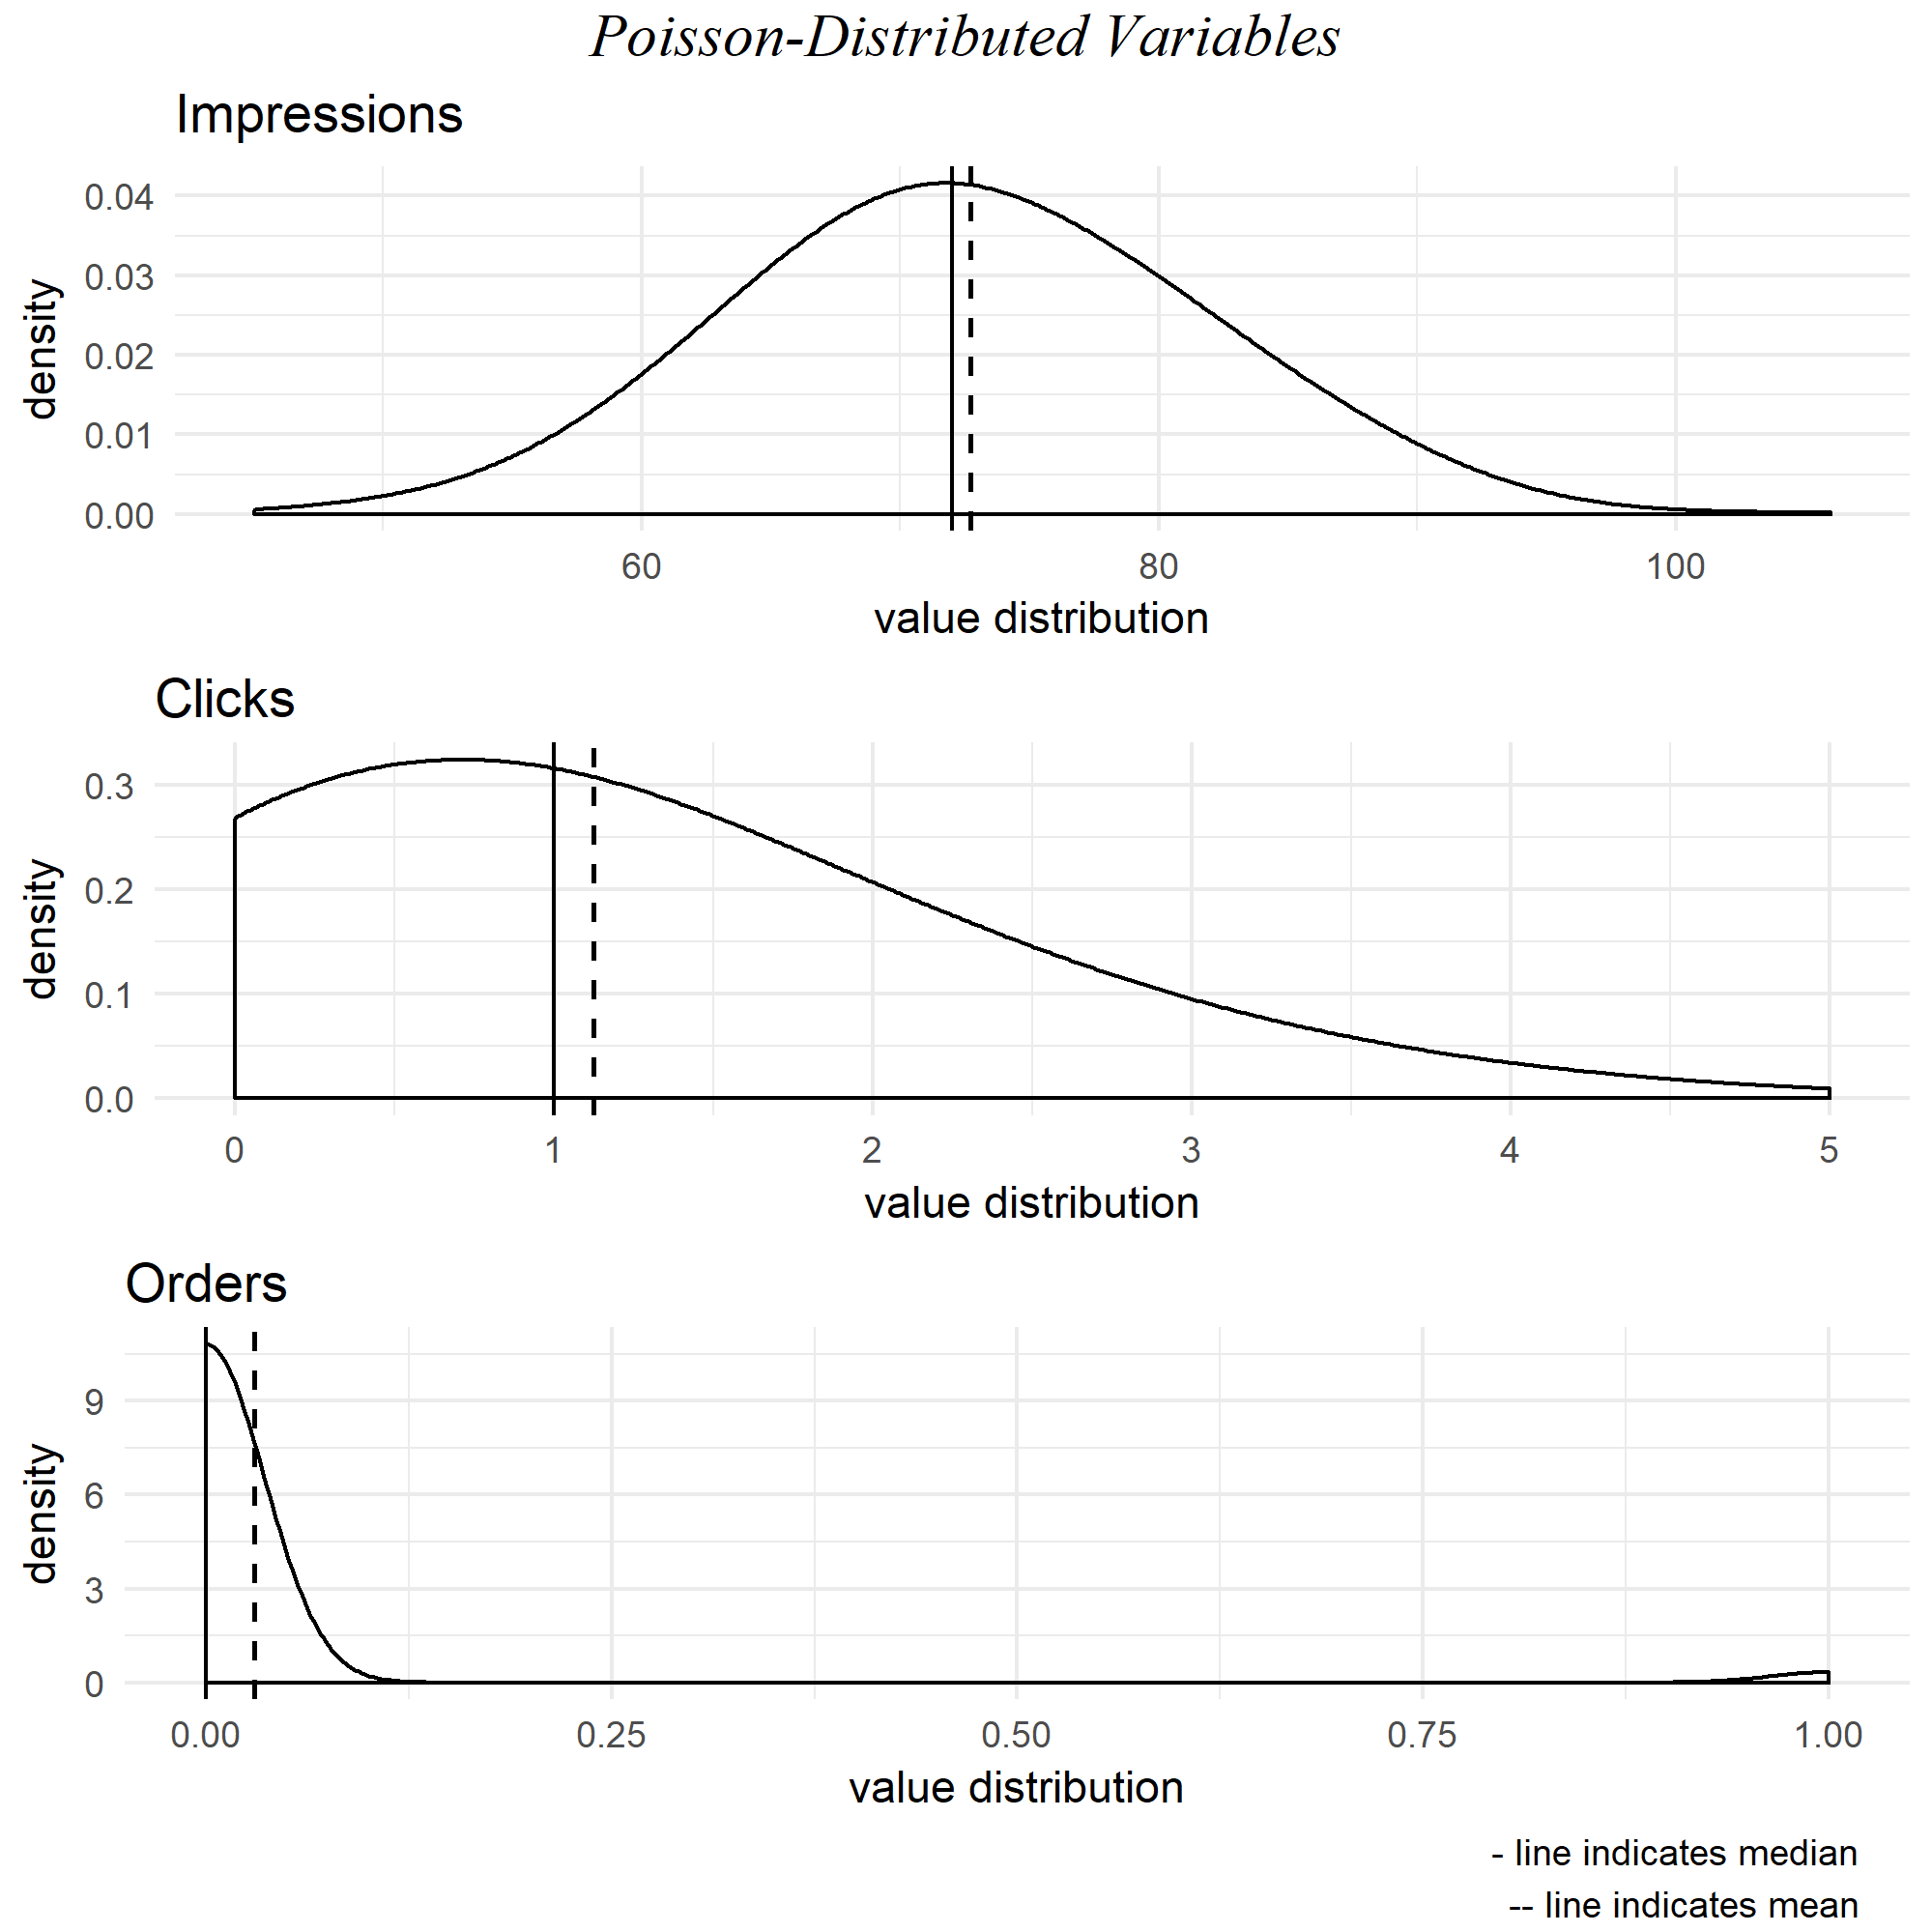
\includegraphics[scale = 0.7]{poisson_plots.png}
    \caption{Distributions for the three Poisson-distributed variables}
    \label{fig:Poission}
\end{figure}
Although it may appear to be normally distributed, the distribution for Impressions is, in fact, a Poisson distribution. To be in line with the min and max values established in the summary statistics table, any values below 1 and above 1666 (min and max, respectively), if any, have been replaced by the min and max values themselves. 
The Clicks distribution peaks close to 1 and gently slopes downward to 5, which logically makes sense as users would most often click 0 to 1 times on any particular ad in one user session. As with Impressions, Clicks has established min and max values - 0 and 24 - and any values outside of this range were replaced with the min/max values as appropriate\footnote{It is not possible, at least as far as we are aware, for a user to make -1 clicks!}.\\
Finally, the Orders distribution is bimodal, with a large peak at 0 and a much smaller peak at 1. This distribution is a bit misleading as a user can only either place an order or not, hence the 0-1 peaks. One may consider this more a binomial variable, but we chose to model it as Poisson because it is an event that occurs potentially at random and across an unknown time interval.\\
The Orders variable also has minimum- and maximum-allowed values, these being 0 and 3, respectively (as with clicks, a user cannot make a negative order).

\subsubsection{Binomial-Distributed Variables}
The three binomial variables are relatively simple in their usage, in that they represent whether an event occurred or not. Each of these variables act as a sort of on/off switch for the inclusion of the parameters in the simulation for a particular keyword at a particular time.
\begin{figure}[!h]
    \centering
    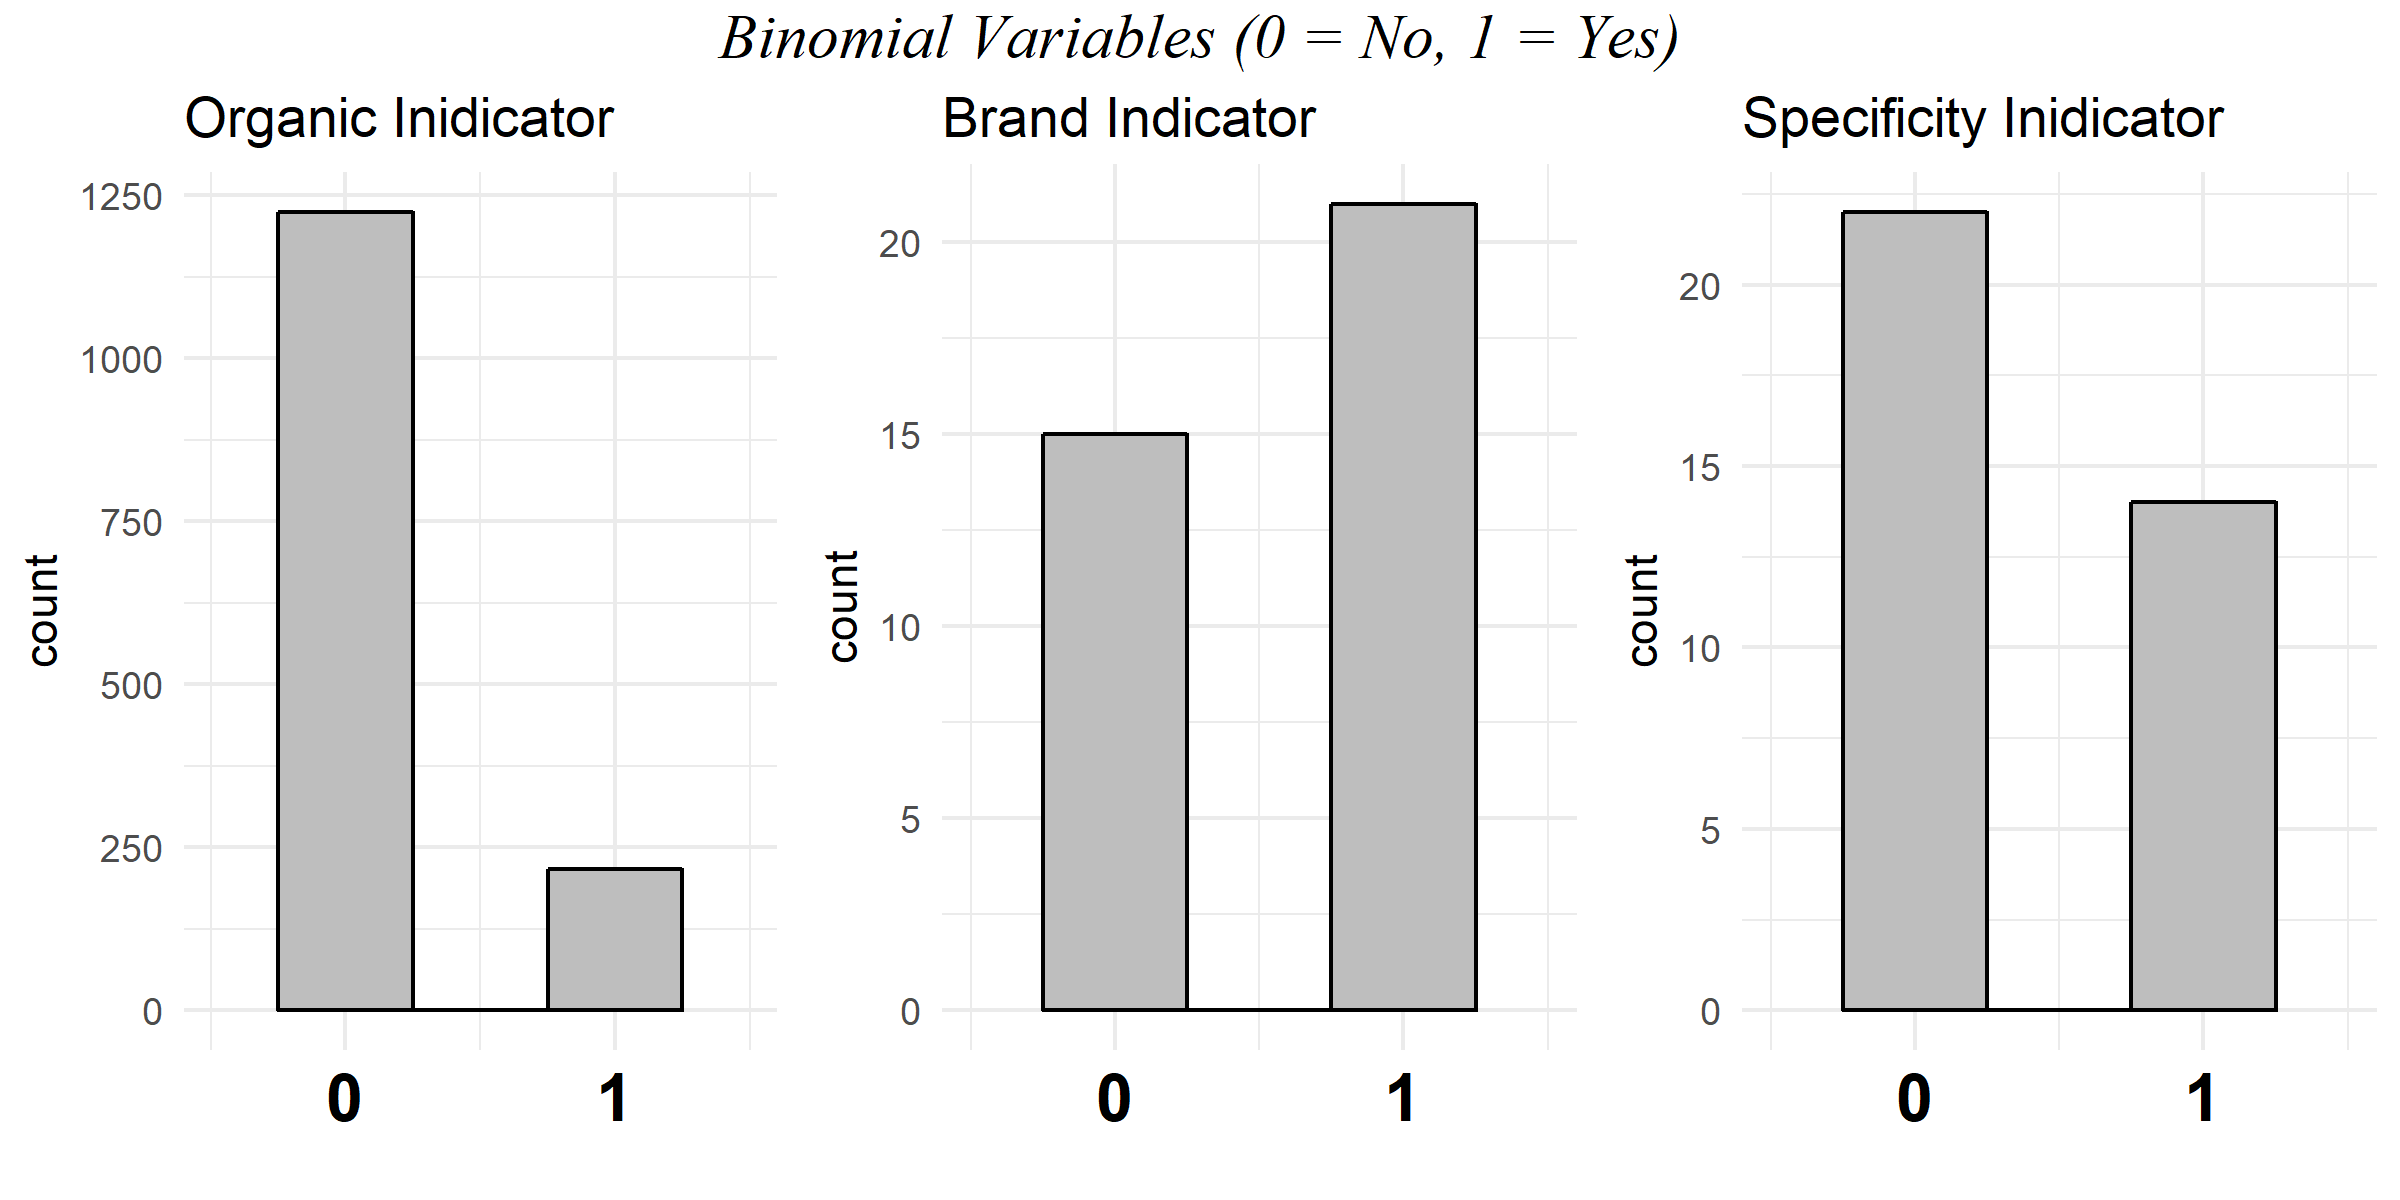
\includegraphics[scale = 0.6]{binomial_plots.png}
    \caption{Distributions for the three Binomial-distributed variables}
    \label{fig:Binomial}
\end{figure}
As mentioned in the paper, Organic is "a dummy variable which is set to one if the advertiser's organic listing appears on the first page, and is set to zero otherwise"\citep[p. 20]{agarwal_organic_2015}. Similarly, Brand is an indicator variable which is set to 1 if a known brand name is in the keyphrase used in the experiment, and is 0 if a brand name is not included.\\
Specificity is a bit more involved - this is actually an indicator of which level in the resulting website's site hierarchy the user reaches when routed through the search engine (i.e., how close to the actual searched-for product does the user get when they click on the link in the search engine?). For example, the specificity for a generic keyword - the authors mention 'pet food' - is 0, while a more specific keyword, such as 'dog food', is scored as a 1 \citep{agarwal_organic_2015}. The paper mentions the possibility for values greater than 1, but the maximum value for specificity given in the summary statistics table is 1, so we chose to model this variable as binomial.

\subsubsection{Normally Distributed Variables}
As might be expected, the predominance of our simulated variables follow a normal distribution.\\ 
\begin{figure}[!h]
    \centering
    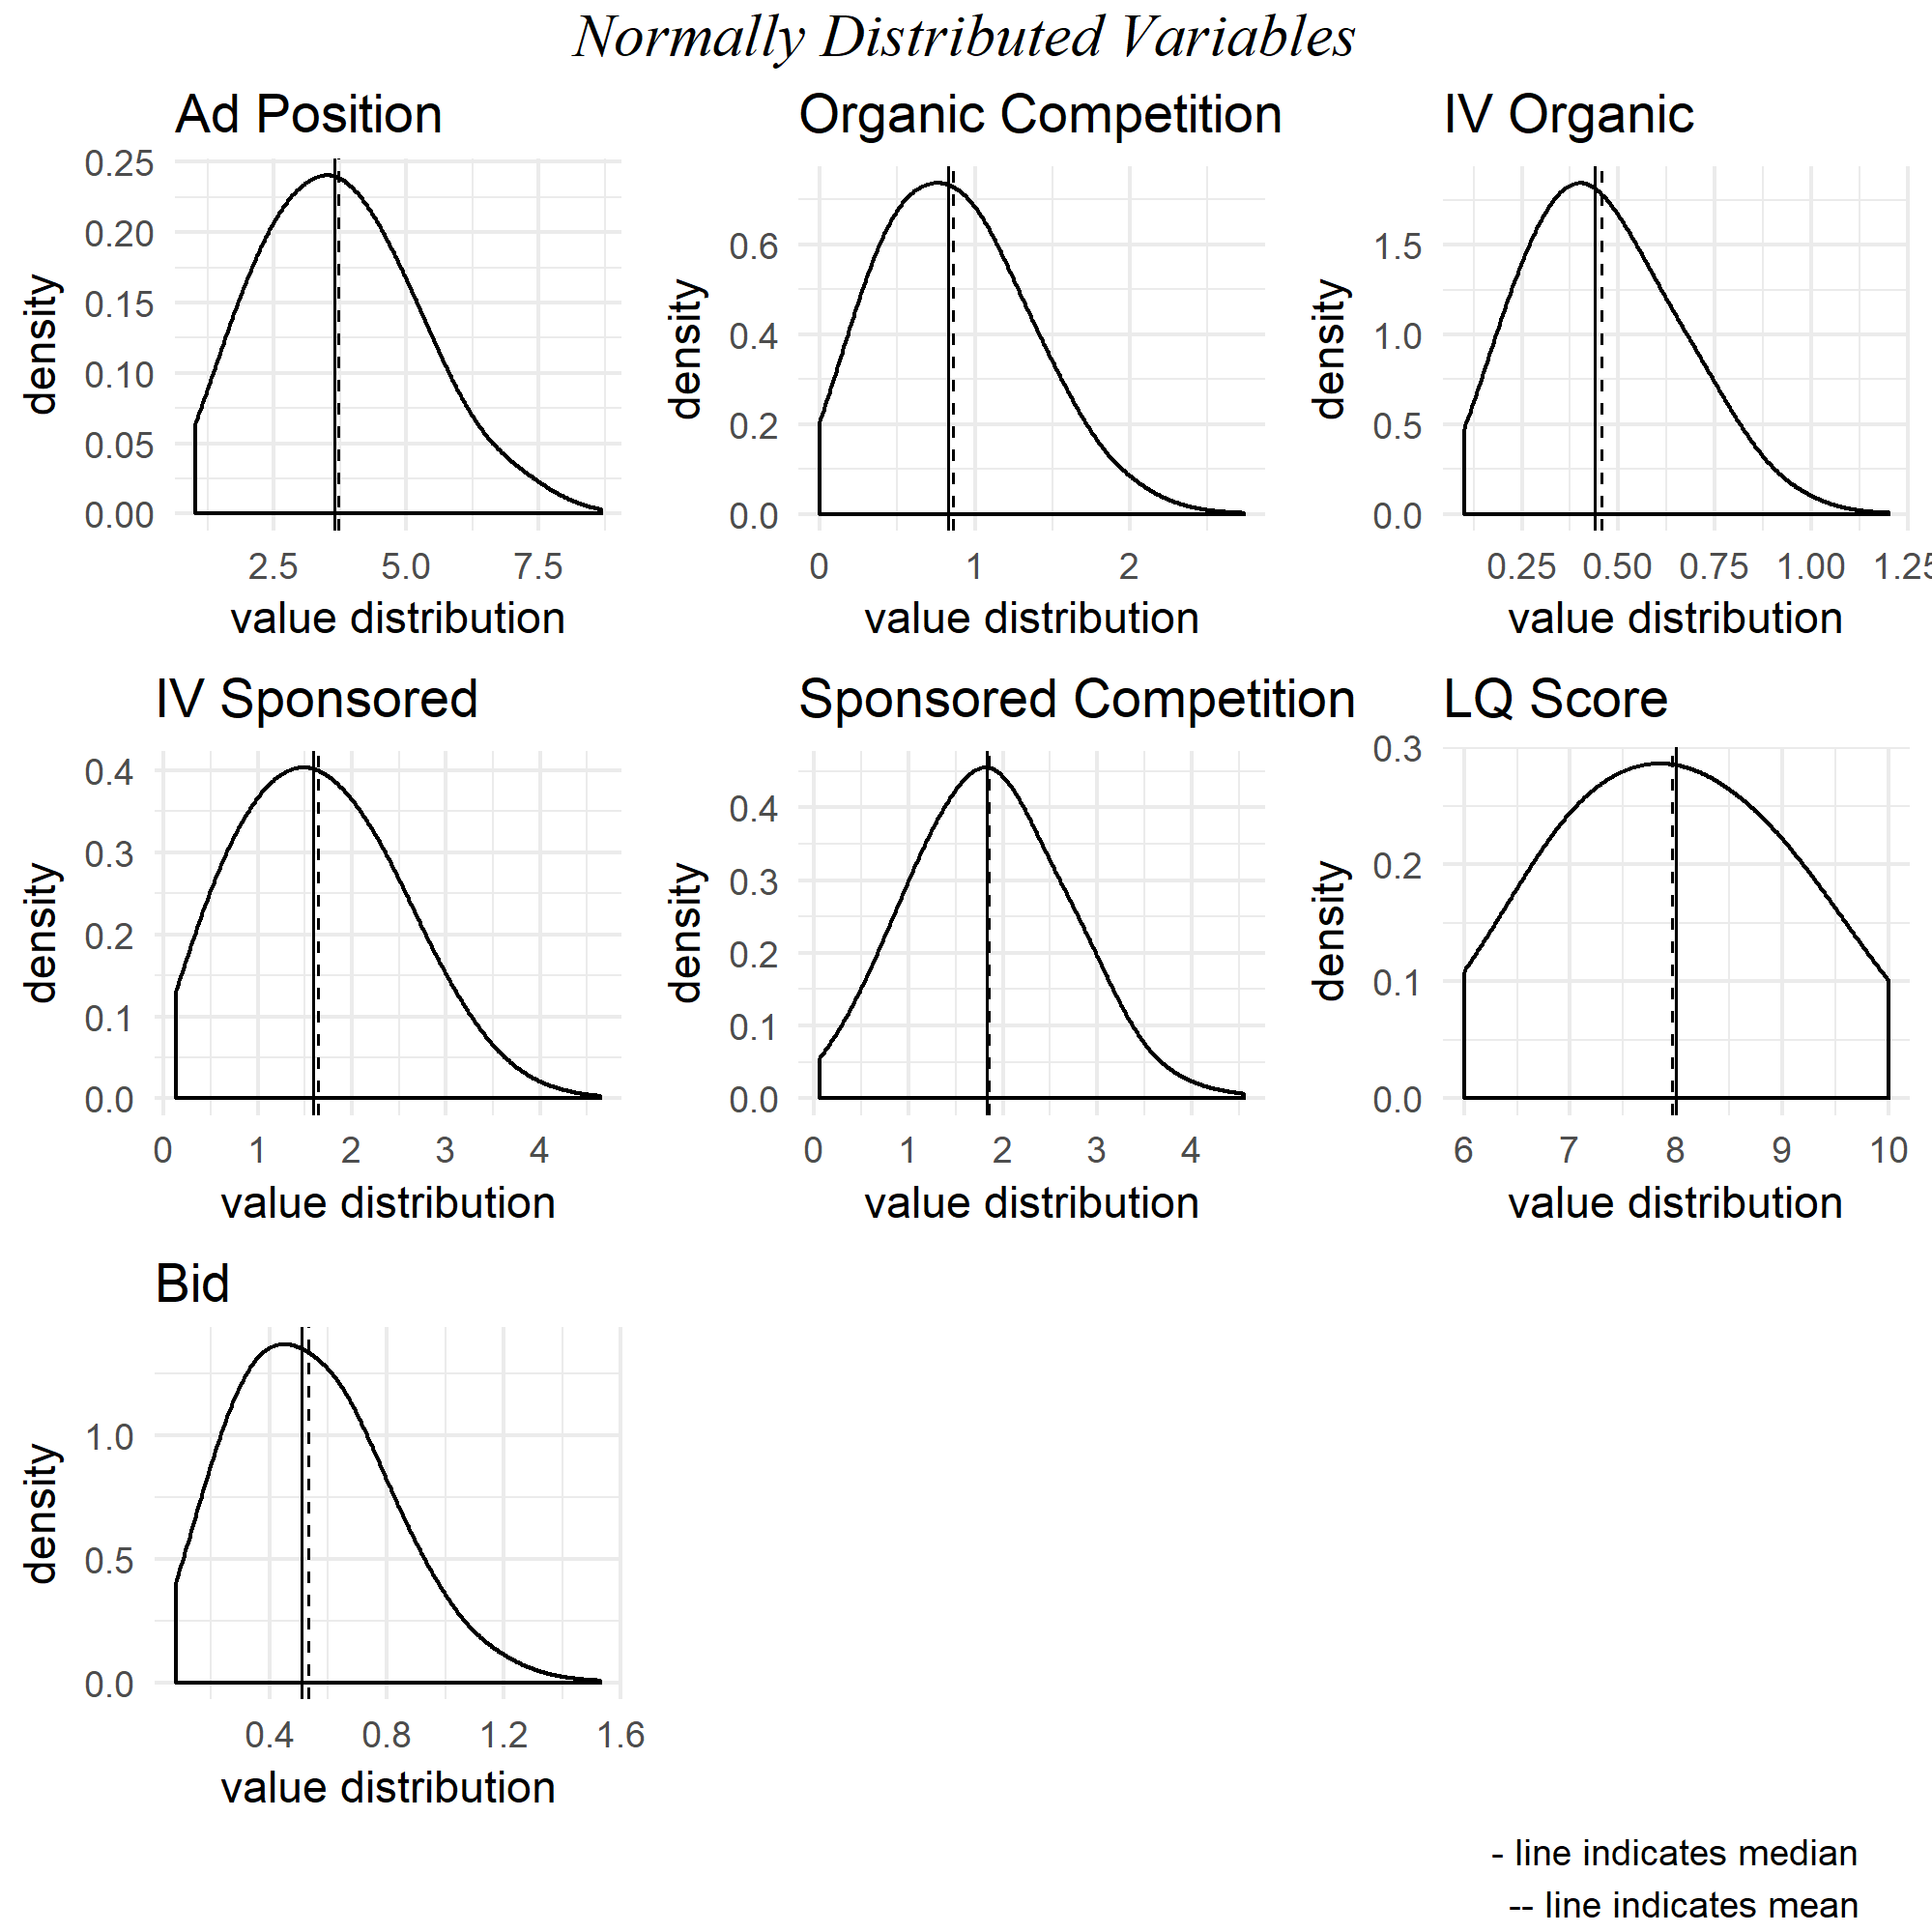
\includegraphics[scale = 0.72]{normal_plots.png}
    \caption{Distributions for the seven Normally distributed variables}
    \label{fig:Normal}
\end{figure}
It is not necessary to get into the specifics of each variable, save it to point out a few noticeable oddities about the graphs. As can be seen in figure \ref{fig:Normal}, both the mean and median are slightly right-of-center for all of the variables simulated. This is due to the fact that all of the normal distributions are \textit{truncated} normal distributions. for all but the LQ score, the minimum value given for each variable in the summary statistics table is 0; that is, the simulation would have produced values less than 0 had the minimum value in the code used not been set at 0. LQ score is even more truncated, with limits placed on its left and right tails at 6 and 10, respectively (6 being the minimum score found in the data statistics, and 10 being the maximum value allowed in the LQ scoring system).

\newpage
\subsection{Simulating the parameters of the model}
\subsubsection{The $\theta^k$s}
\begin{figure}
    \centering
    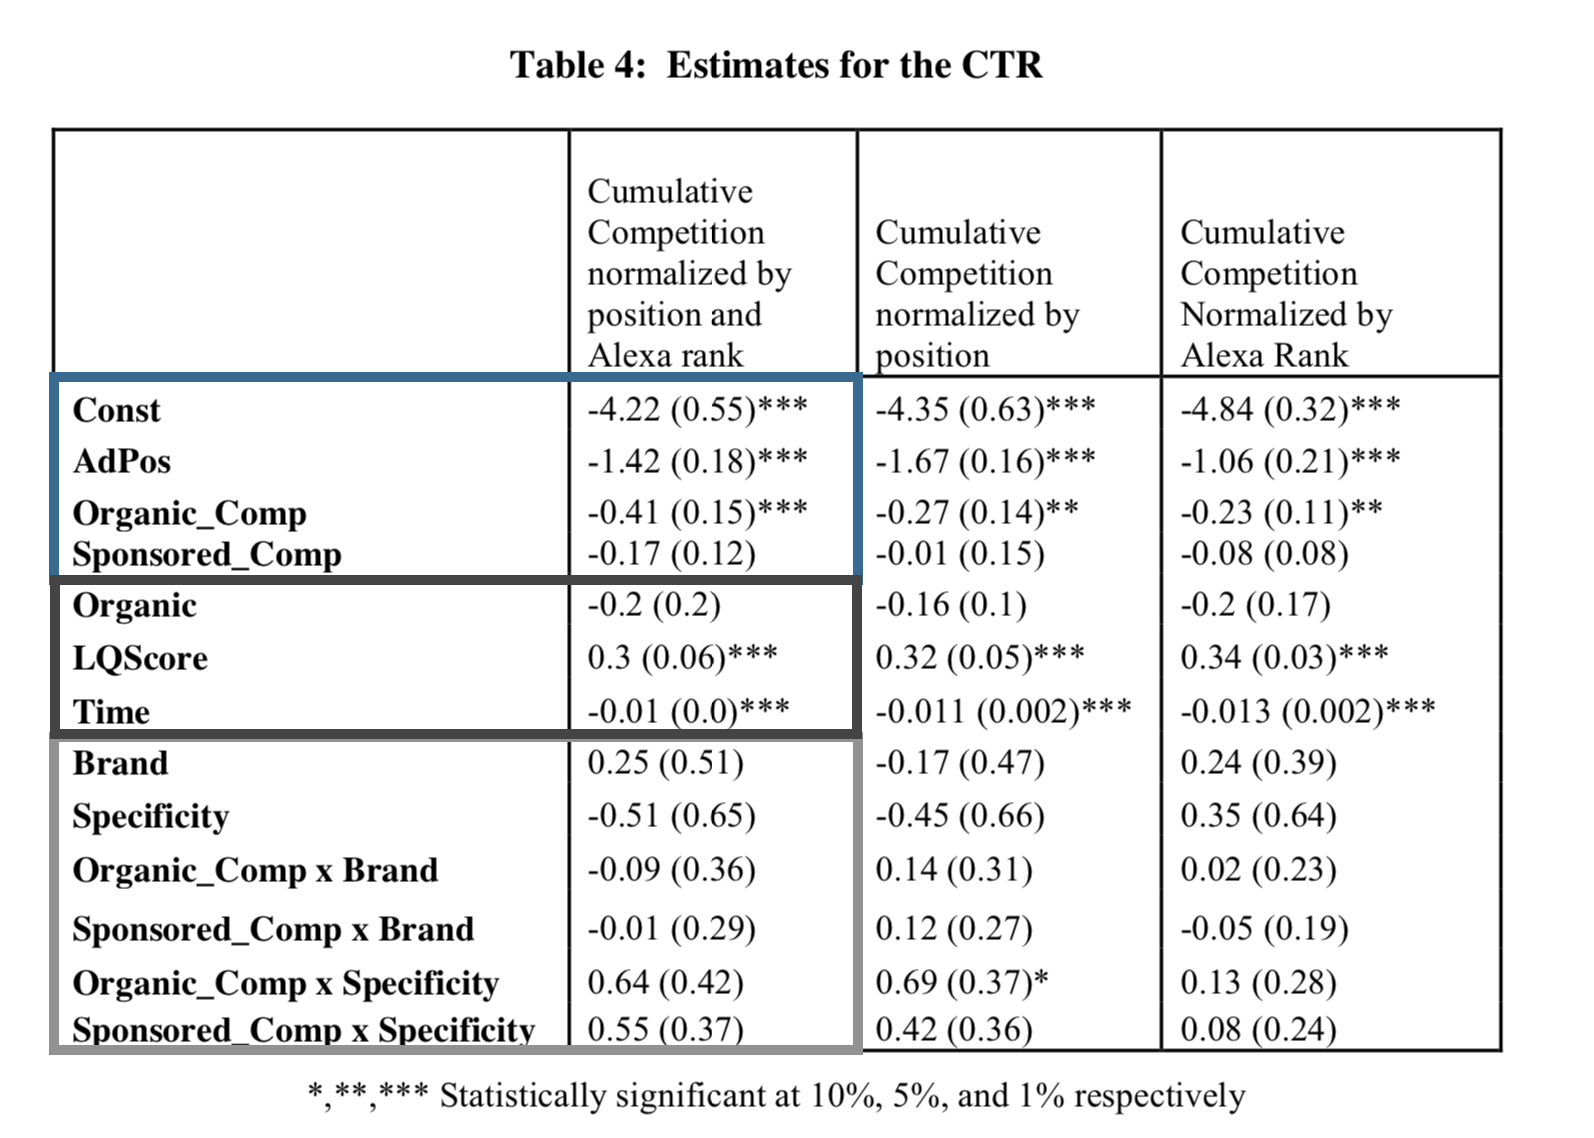
\includegraphics[scale=0.35]{table4}
    \caption{The estimates for CTR from p. 39. The authors' estimates for the $\theta^k$s in dark blue are only used for comparison. The values marked in dark grey served as constants for $\theta_4, \theta_5$ and $\theta_{Time}$. The light grey box refers to the $\Delta^{\theta}$ matrix in the code, denoted as \texttt{theta\_delta}\protect\footnotemark.}
    \label{fig:table4}
\end{figure}
\footnotetext{"Brand" and "specificity" was interpreted as $\theta_0$ x brand or specificity. As $\theta_1$,the bias for $AdPos_{kt}$, is missing it is assumed to be 0. Though $\Delta^{\theta}$ is constant for all k, the standard deviation might refer to the variation throughout the MCMC chain.}

After sampling the data, the hierarchical model's parameters needed to be estimated. Figure \ref{fig:table4} depicts how the data given was interpreted as not all values relate to a clearly identifiable part in the introduced model.\\
Essentially, the parameters from the linear model dependent on k have been drawn from a multivariate distribution with a mean $\Delta^{\theta}z_k$ specifying its relationship with the keyword specifics and a sigma matrix $V^{\theta}$. While $\Delta^{\theta}z_k$ has been taken from figure \ref{fig:table4}, $V^{\theta}$ was sampled from an Inverse Wishart distribution with 4 degrees of freedom and an identity matrix.\footnote{The matrix given in equation \ref{eq:vmatrix} is recursively defined and has thus been neglected in this section. See the estimation, section \ref{sec:estimation}, for further details.} In a sense, $V^{\theta}$ serves as a matrix for the error within the estimates of one parameter, so how the different factors come into play for the CTR. The code uses \texttt{theta\_delta} as $\Delta^{\theta}$, \texttt{VTheta} as $V^{\theta}$ and \texttt{random\_thetas} as the 4 $\theta^k$s.\\

\newpage
\begin{lstlisting}[caption={Code for simulating $\Delta^{\theta}$ and $V^{\theta}$.}]
# The theta_delta matrix is given incompletely, all missing values are treated as 0. It is all parameters depending on k in interaction with a keyword's brand and specificity, giving a 4x2 (or 2x2) matrix.
theta_delta <- matrix(c(c(0.25, -0.51), # const x brand and spec
                        c(0,0), # adpos x brand and spec
                        c(-0.09, 0.64), # organic_comp x brand and spec
                        c(-0.01,0.55)), # sponsored_comp x brand and spec
                      nrow=4, ncol=2, byrow=TRUE)
                      
# The covariance matrices: basically the error "within" a set of parameters 4 thetas depend on k, so VTheta is 4x4. All in all, there are 4 V matrices, one for each parameter set, two of size 4x4, two of size 2x2.
VTheta <- riwish(4, diag(1,nrow=4))

# Define the function to draw the parameters dependent on k
# It first simulates the u_error and then takes the delta_matrix times the z vector.
calc_coeff_matr <- function(keywords, delta_matr, z, v_matr) {
  l = matrix(nrow= 4, ncol=keywords)
  for (k in 1:keywords){
    u <- matrix(rmvnorm(n=1, mean=rep(0,nrow(delta_matr)), v_matr),
                nrow=nrow(delta_matr))
    d <- delta_matr %*% z[[k]] + u
    l[,k] <-  d
  }
  return(l)
}

# The thetas dependent on k for CTR
random_thetas <- calc_coeff_matr(num_keywords, theta_delta, z, VTheta)

# Took the mean values for the thetas that do not depend on k.
theta4 <- -0.2; theta5 <- 0.3; theta6 <- -0.01
\end{lstlisting}

\newpage
\subsubsection{The error terms $\epsilon^{\theta}_{kt}$ of the linear model}
As $V^{\theta}$ denotes the error within the different $\theta^k$s, $\Omega$ accounts for correlated error terms among $\theta$, $\beta$, $\alpha$ and $\gamma$. Based on the numbers in figure \ref{fig:errorterms}, $\Omega$ is the sigma matrix for the draw of the 4 kxt error matrices $\epsilon$ from the multivariate normal distribution, see equation \ref{eq:omega}.\\

\begin{lstlisting}[caption={Code for generating the error terms.}]
#------------calculate the error terms-------------------#
r1 <- c(0.370,	-0.036,	0.000,	-0.005)
r2 <- c(-0.036,	0.232,	0.007,	0.02)
r3 <- c(0,	0.007,	0.064,	-0.005)
r4 <- c(-0.005,	0.02,	-0.005,	0.087)

o_mat_cols <- c('CONV','CTR','Pos','Organic_comp')
omega_matrix <- matrix(c(r1, r2, r3, r4), nrow=4, ncol=4, byrow=TRUE, dimnames = list(o_mat_cols))
colnames(omega_matrix) <- o_mat_cols

error_terms <- rmvnorm(n = num_observations, sigma=omega_matrix)
errors <- vector(mode="list", length=4)
names(errors) <- c('theta_error','beta_error','gamma_error','alpha_error')
errors[[1]] <- matrix(error_terms[,1], nrow=num_keywords, ncol=num_days)
# [errors[[2]] till 4 in the same manner]

theta_error <- errors$theta_error
\end{lstlisting}
\begin{figure}[h!]
    \centering
    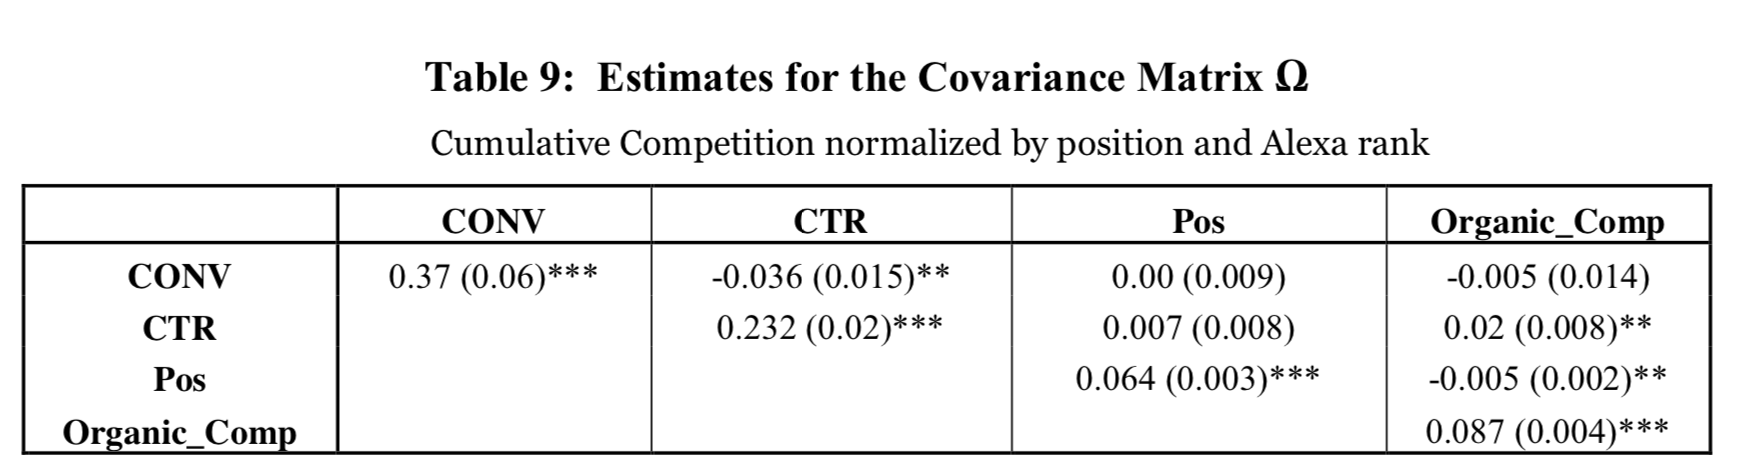
\includegraphics[scale=0.35]{errorterms}
    \caption{Table 9 from the paper, giving estimates for the error terms}
    \label{fig:errorterms}
\end{figure}

\newpage
\subsubsection{The final step towards $\Lambda^{CTR}_{kt}$}
The parameters were then combined into a linear model with the data and the error term $\epsilon^{\theta}_{kt}$, equation \ref{eq:mainlinear}. The resulting utility of clicking $U^{CTR}_{kt}$ represents the latent variable for the click-through rate. The logistic function of $U^{CTR}_{kt}$ finally leads to the dependent variable CTR, the $\Lambda^{CTR}_{kt}$ from equation \ref{eq:lambda} or \texttt{CTR\_estimate} in the code.

\begin{lstlisting}[caption={Code for simulating the parameters, shown for $\theta$.}]
# The final linear model
u_ctr <- matrix(nrow=num_keywords, ncol=num_days)
CTR_estimate <- matrix(nrow=num_keywords, ncol=num_days)
for (t in 1:num_days) {
  for (k in 1:num_keywords){
    u_ctr[k,t] <- random_thetas[[k]][1] + random_thetas[[k]][2]*adpos_eq[k,t] +
      random_thetas[[k]][3]*orgcomp_eq[k,t] + random_thetas[[k]][4]*sponsored_comp[k,t] +
      theta4*organic[k,t] + theta5*lqscore[k,t] +
      theta6*t + theta_error[k,t]
      
    CTR_estimate[k,t] <- exp(u_ctr[k,t]) / (1 + exp(u_ctr[k,t]))
    # the logit part
    }
}
# [same for betas, gammas and alphas]

\end{lstlisting}

\subsection{Simulation and Summary Statistics Comparison}
The end result of our simulation is the estimation of the CTR and CONV, ideally to be comparable to those found by the authors themselves. To compare our simulation outcome with the estimation from the paper, we first calculated the CTR and CONV based on the summary statistics given in the paper. The mean values for these are shown in table \ref{table:ctr-conv-vs}.

\begin{center}
\begin{table}[h!]
 \begin{tabular}{|c|c|c|c|c|}
 \hline
  & CTR Paper & CTR Simulation & CONV Paper & CONV Simulation \\
 \hline
 Mean & 0.01553 & 0.67544 & 0.00026 & 0.36571\\ 
 \hline
 Median & 0.01369 & 0.90372 & 0 & 0.02198 \\
 \hline
\end{tabular}
\caption{Mean and median values of simulated and paper-estimated CTR and CONV rates.}
\label{table:ctr-conv-vs}
\end{table}
\end{center}

As is apparent in \ref{table:ctr-conv-vs}, our simulation produced both CTR and CONV rate estimates with a much higher mean and median value than the summary statistics in the paper would suggest. Examining the distribution of the data helps to make the estimates we generated more understandable. 
\begin{figure}[!h]
    \centering
    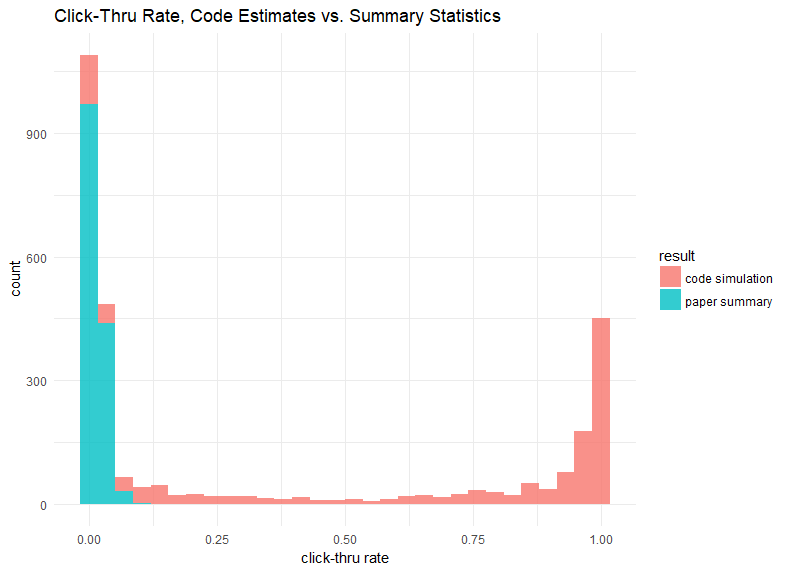
\includegraphics[scale = 0.65]{ctr_sim_code_plot.png}
    \caption{Count of simulated and summary statistic-based CTR estimates}
    \label{fig:CTR}
\end{figure}

Figure \ref{fig:CTR} shows that our simulation and the summary statistic-generated data do trend heavily toward 0, although out simulated data includes a much wider variety of possible click-through rates, as well as a great deal hovering around 1. While we did our best to follow the equations and formulas given in the paper, it is possible that we either mistakenly coded something, or that a piece of necessary information was missing in the paper itself\footnote{As mentioned, there seem to have been several noticeable omissions in the data needed to fully replicate the paper.}.

\begin{figure}[!h]
    \centering
    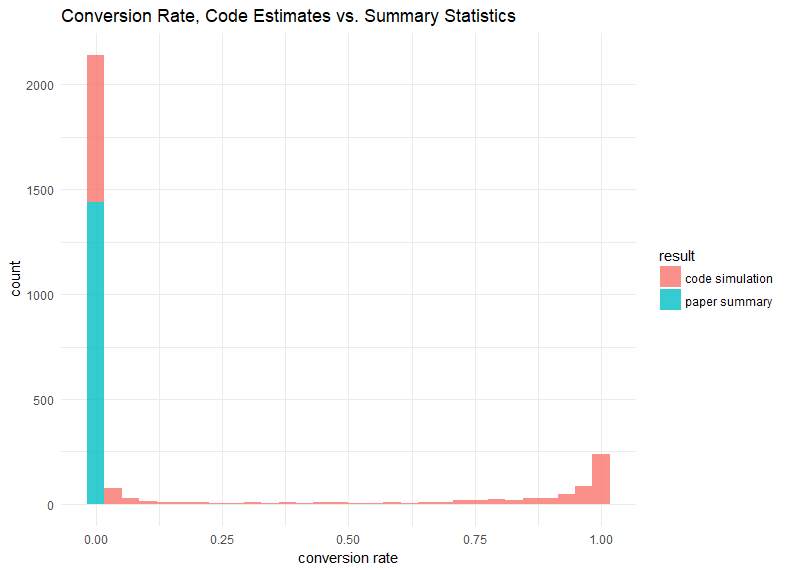
\includegraphics[scale = 0.6]{conv_sim_code_plot.png}
    \caption{Count of simulated and summary statistic-based CONV estimates}
    \label{fig:CONV}
\end{figure}

The simulated conversion rate follows a similar pattern as that of the click-through rate, as is clear in figure \ref{fig:CONV}. In keeping in line with the summary statistics data, our simulated data does trend around 0, yet, we again see a much greater distribution of data points in the simulated data. The spread does, however, seem to be less pronounced with the conversion rate than with the click-through rate.
